\section{Trees}\label{s:k-ary_trees}
When analyzing a general problem of graph drawings, the class of trees is of interest due to their assessable properties. The first graph class considered for minimizing the ratio in a drawing is therefore the class of $k$-ary trees. The results of this class of trees will be applicable to any rooted tree. This section describes a drawing algorithm for a $k$-ary tree $T$, guaranteeing a nearly optimal Euclidian ratio in the resulting drawing $\Gamma_T$. The total area of $\Gamma_T$ will depend on the height of $T$.\\
% properties of complete k-ary trees
Trees are connected and acyclic per definition, inheriting exactly $n-1$ edges. These properties make trees accessible for a straightforward solution for a given problem.\\
% context for outerplanar graphs
When working on other graph classes, it may be possible to find an approach by reducing a graph $G$ to an instance of a tree. In fact, the resulting drawing algorithm for $k$-ary trees in this section will serve as a first approach for drawing maximal outerplanar graphs in the succeeding section.
\subsection{Properties Of Complete $k$-ary Trees}
\begin{lemma}\label{l:tree_to_k-ary}
	Any tree $T$ can be interpreted as a $k$-ary tree.
\end{lemma}
A tree $T$ does not necessarily inherit a root but any vertex of $T$ can be flagged as such. The height of any vertex is then described as the path length starting from the root and $k$ is set to the maximum amount of children of all the inner nodes. $T$ is now rooted and $k$ fixed, hence a $k$-ary tree. When describing a tree $T$ as a $k$-ary tree, the root will be chosen so the resulting height is minimal.
% The height 
\begin{lemma}The \emph{height $h$} of a complete $k$-ary tree $T$ is in $\mathcal{O}(\log n)$.\label{l:k-ary-tree_log_height}
\end{lemma}
\begin{proof}
	\begin{align}
		n = \sum_{i=0}^{h}k^i &= \frac{k^{h+1}-1}{k-1}\\
		\Leftrightarrow h &= \log_k((k-1)n+1)-1\\
		&= \frac{\log((k-1)n+1)}{\log k}-1\\
		\underbrace{\Rightarrow}_{k \text{ fixed}}h &\in O(\log n)
	\end{align}
\end{proof}

\subsection{Drawing Algorithm For Complete $k$-ary Trees}

% Drawing result

\begin{theorem}
	There exists a linear-time drawing algorithm which produces a planar straight-line drawing for complete $k$-ary trees with a nearly optimal ratio, apart from a rounding error, on area $\mathcal{O}(n^2\log n)$.
\end{theorem}
\begin{proof}
	The following drawing will be constructed from top to bottom, meaning that the $y$-coordinates of the children of any vertex $v$ are smaller than the $y$ coordinate of $v$.\\
	Let $r := k^h$. For a vertex $v$ in height $i$, consider $k$ equidistant columns with $x$-coordinates between $x(v) - (k-1)\cdot  k^{h-h'-1}$ and $x(v) + (k-1)\cdot  k^{h-h'-1}$. These are integer coordinates since the distance between two columns next to each other equals $2\cdot \frac{k^{h-i}}{k}$. Draw a circle around $v$ with radius $r$. Choose the grid points $v_i$ on the column closest to the resulting intersections with the constraint that $y(v_i) \leq y(v)$ and connect $v$ with its $k$ children with a straight-line.
\begin{figure}[H]
	\centering
		\begin{subfigure}{\textwidth}
			\centering
			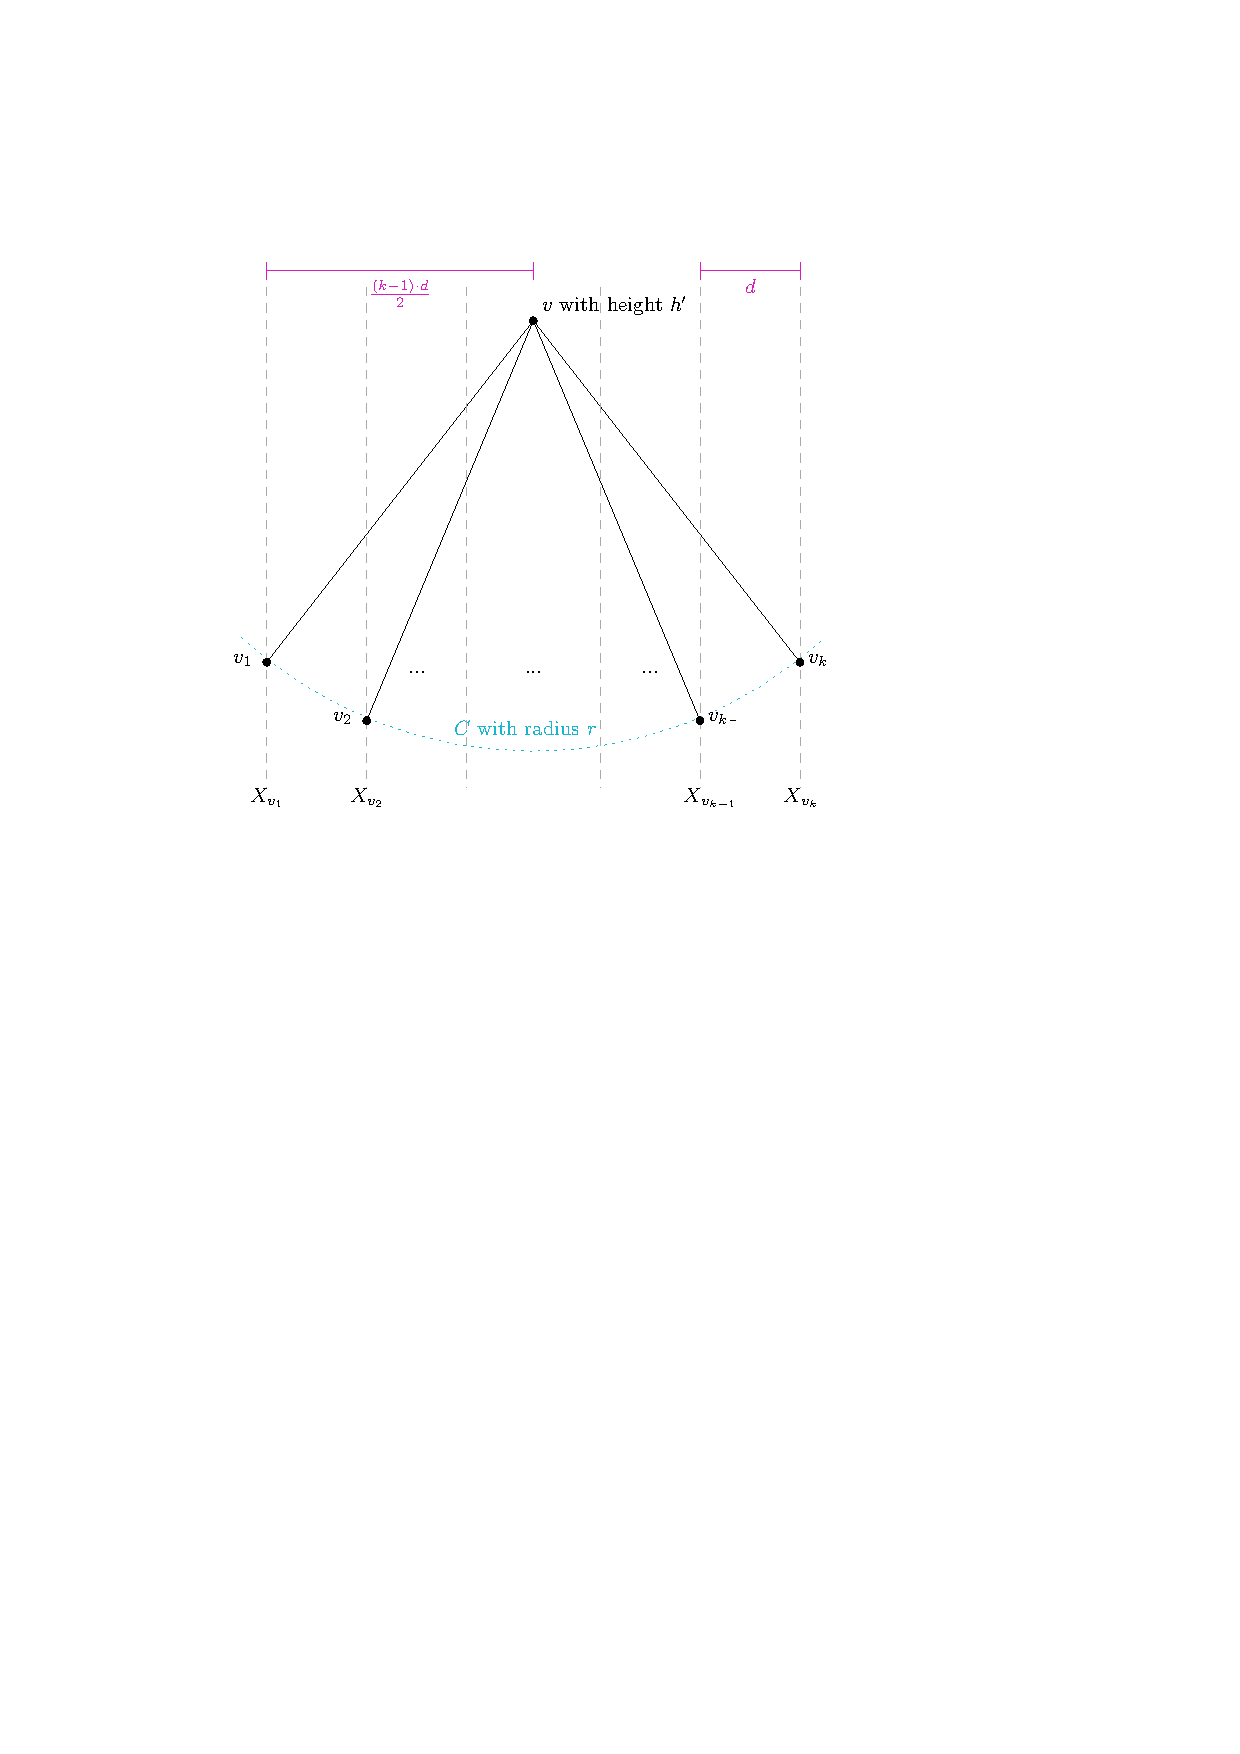
\includegraphics[page=1,width=0.6\linewidth]{graphics/k-ary_tree_algorithm_construction.pdf}
		\end{subfigure}
	\caption{Illustration of drawing algorithm at a vertex $v$ with height $h$}\label{im:k-ary_trees_algorithm_illustration}
\end{figure}
	The distance between two neighbouring columns in height $i$ suffices for the remaining drawing since it holds for the remaining heights:
	\begin{align}
		\underbrace{2\cdot \sum_{j=i}^{h-1} k^{h-j-1}}_{\text{drawn from both columns}} &= 2\cdot\sum_{z = 0}^{h-i-1}h^z\\
		&= 2\cdot\frac{k^{h-i}-1}{k-1} < 2\cdot k^{h-i}
	\end{align}
	The height of the drawing is bound by $h\cdot r = h\cdot k^h \in \mathcal{O}(n\cdot \log n)$. The width is bounded by $2\cdot\sum_{i = 0}^{h} k^i = 2\cdot \frac{k^{h+1}-1}{k-1} \in \mathcal{O}(n)$, resulting in $\mathcal{O}(n^2\log n)$ area.\\ 
	Since the algorithm works from top to bottom and for height $i$, the area for every subtree is disjointedly reserved, the resulting drawing is planar. Furthermore, all straight-line edges inherit a length of approximately $k^h$. A rounding error bound by $\varepsilon, 0\leq \varepsilon<1$ occurs when placing the vertices on grid points. The rounding error does not accumulate since the length $r$ is fixed and the vertices are placed in the grid independently from each other. No bends were used and the ratio is bound by $1+\varepsilon$.
\end{proof}
\bigskip
The following drawing algorithm sums up the approach described above.\\
\begin{algorithm}[H]
	\KwIn{complete $k$-ary tree $T$, $h$}
	\KwOut{Straight-line drawing of $T$ with nearly optimal ratio}
	\caption{Draw\_$k$-ary\_tree($T$)}\label{al:complete_k-ary_tree}
	$h \gets $ \text{height of $T$}\\
	$r \gets k^h$\\
	Draw $root(T)$ on any grid point\\
	\texttt{Draw\_$k$-ary\_Children}$(root(T),r,h)$\\
	\Return $\Gamma$
\end{algorithm}
\begin{algorithm}[H]
	\KwIn{Already drawn vertex $v$, radius and height $r,h \in \mathbb{N}$}
	\KwOut{Coordinates of all the children of $v$}
	\caption{\texttt{Draw\_$k$-ary\_Children}$(v,r,h)$}
	\If{$v$ leaf}{\Return}
	\Else{
		$h' \gets \texttt{height}(v)$\\
		$d \gets 2\cdot k^{h-h'-1}$\\
		$C \gets \Gamma.\texttt{DrawCircle}(r,v)$\\
		\tcc{Draw circle with radius $r$ around $v$}
		\For{$i \in [1..k]$}{
			$x(v_i) \gets x(v) - \frac{(k-1)\cdot d}{2} + (i-1)\cdot d$\\
			\tcc{$x$-coordinate of $i$-th child of $v$}
			$X \gets \Gamma.\texttt{Column}(x(v_i))$\\
			\tcc{Identify the column at position $x(v_i)$}
			$s \gets \Gamma.\texttt{Intersection}(I,X)$\\
			\tcc{Calculate the intersection of the circle $C$ and the column $X$}
			$y(v_i) \gets round(y(s))$\\
			$\Gamma.$\texttt{DrawStraightLine}$(v,v_i)$\\
			$\Gamma.$\texttt{Draw\_$k$-ary\_Children}$(v_i,r,h)$
		}
	}		
\end{algorithm}

\subsection{Drawing Algorithm For General Trees}

\begin{theorem}
	Any tree $T$ admits a optimal straight-line drawing, apart from a rounding error, on exponential area.
\end{theorem}
\begin{proof}
	By Lemma \ref{l:tree_to_k-ary}, any tree $T$ can be interpreted as a $k$-ary tree. The algorithm \ref{al:complete_k-ary_tree} can be reused in order to produce a nearly-optimal straight-line drawing. Set the root $r \in V(T)$ so that the height of $T$ is minimal. Set $k$ as the maximum amount of children of all inner nodes of $T$. The drawing algorithm \ref{al:complete_k-ary_tree} is slightly modified which checks the existence of any vertex since any $k$-ary subtree with height $h$ is a subtree of a complete $k$-ary subtree of the same height. The output will be a nearly-optimal straight-line drawing $\Gamma_{T'}$. Removing the marked vertices will not alter the ratio or area consumption and the result is a nearly-optimal straight-line drawing $\Gamma_T$.
	
	% Consider the following illustration of a tree for the worst case area bounds.
	% TODO figure of worst case tree
	% For this tree, the maximum amount of children as well as the height of $T$ lie in $\mathcal{O}(n)$. The height of the resulting drawing is described as 
\end{proof}

The following drawing algorithm sums up the approach for a general tree $T$.\\
\begin{algorithm}[H]
	\KwIn{A tree $T$}
	\KwOut{Straight-line drawing $\Gamma_T$ with nearly-optimal ratio}
	\caption{Drawing algorithm for a tree $T$}\label{al:general_tree}
	$\texttt{root} \gets v\in V(T)$ with minimal height for $T$\\
	$k \gets 0$
	\For{inner node $v$ of $T$}{
		\If{$v.\texttt{Children.size()} > k$}{
			$k\gets v.\texttt{Children.size()}$
		}
	}
	$h \gets $ \text{height of $T$}\\
	$r \gets k^h$\\
	$\Gamma.\texttt{DrawVertex(root)}$\\
	\tcc{Draw $root(T)$ on any grid point}
	$\Gamma.\texttt{DrawChildren}(\texttt{root},r,h)$\\	
	\Return $\Gamma$
\end{algorithm}

\begin{algorithm}[H]
	\KwIn{Already drawn vertex $v$, radius and height $r,h \in \mathbb{N}$}
	\KwOut{Coordinates of all the children of $v$}
	\caption{\texttt{DrawChildren}$(v,r,h)$}
	\If{$v$ leaf}{\Return}
	\Else{
		$h' \gets \texttt{height}(v)$\\
		$d \gets 2\cdot k^{h-h'-1}$\\
		$C \gets \Gamma.\texttt{DrawCircle}(r,v)$\\
		$q \gets v.\texttt{Children.size()}$\\
		\tcc{Draw circle with radius $r$ around $v$}
		\For{$i \in [1..q]$}{
			$x(v_i) \gets x(v) - \frac{(k-1)\cdot d}{2} + (i-1)\cdot d$\\
			\tcc{$x$-coordinate of $i$-th child of $v$}
			$X \gets \Gamma.\texttt{Column}(x(v_i))$\\
			\tcc{Identify the column at position $x(v_i)$}
			$s \gets \Gamma.\texttt{Intersection}(I,X)$\\
			\tcc{Calculate the intersection of the circle $C$ and the column $X$}
			$y(v_i) \gets round(y(s))$\\
			$\Gamma.$\texttt{DrawStraightLine}$(v,v_i)$\\
			$\Gamma.$\texttt{Draw\_Children}$(v_i,r,h)$
		}
	}		
\end{algorithm}

\subsection{Example Drawings}
\begin{figure}[H]
	\centering
	\begin{subfigure}{\textwidth}
		\centering
		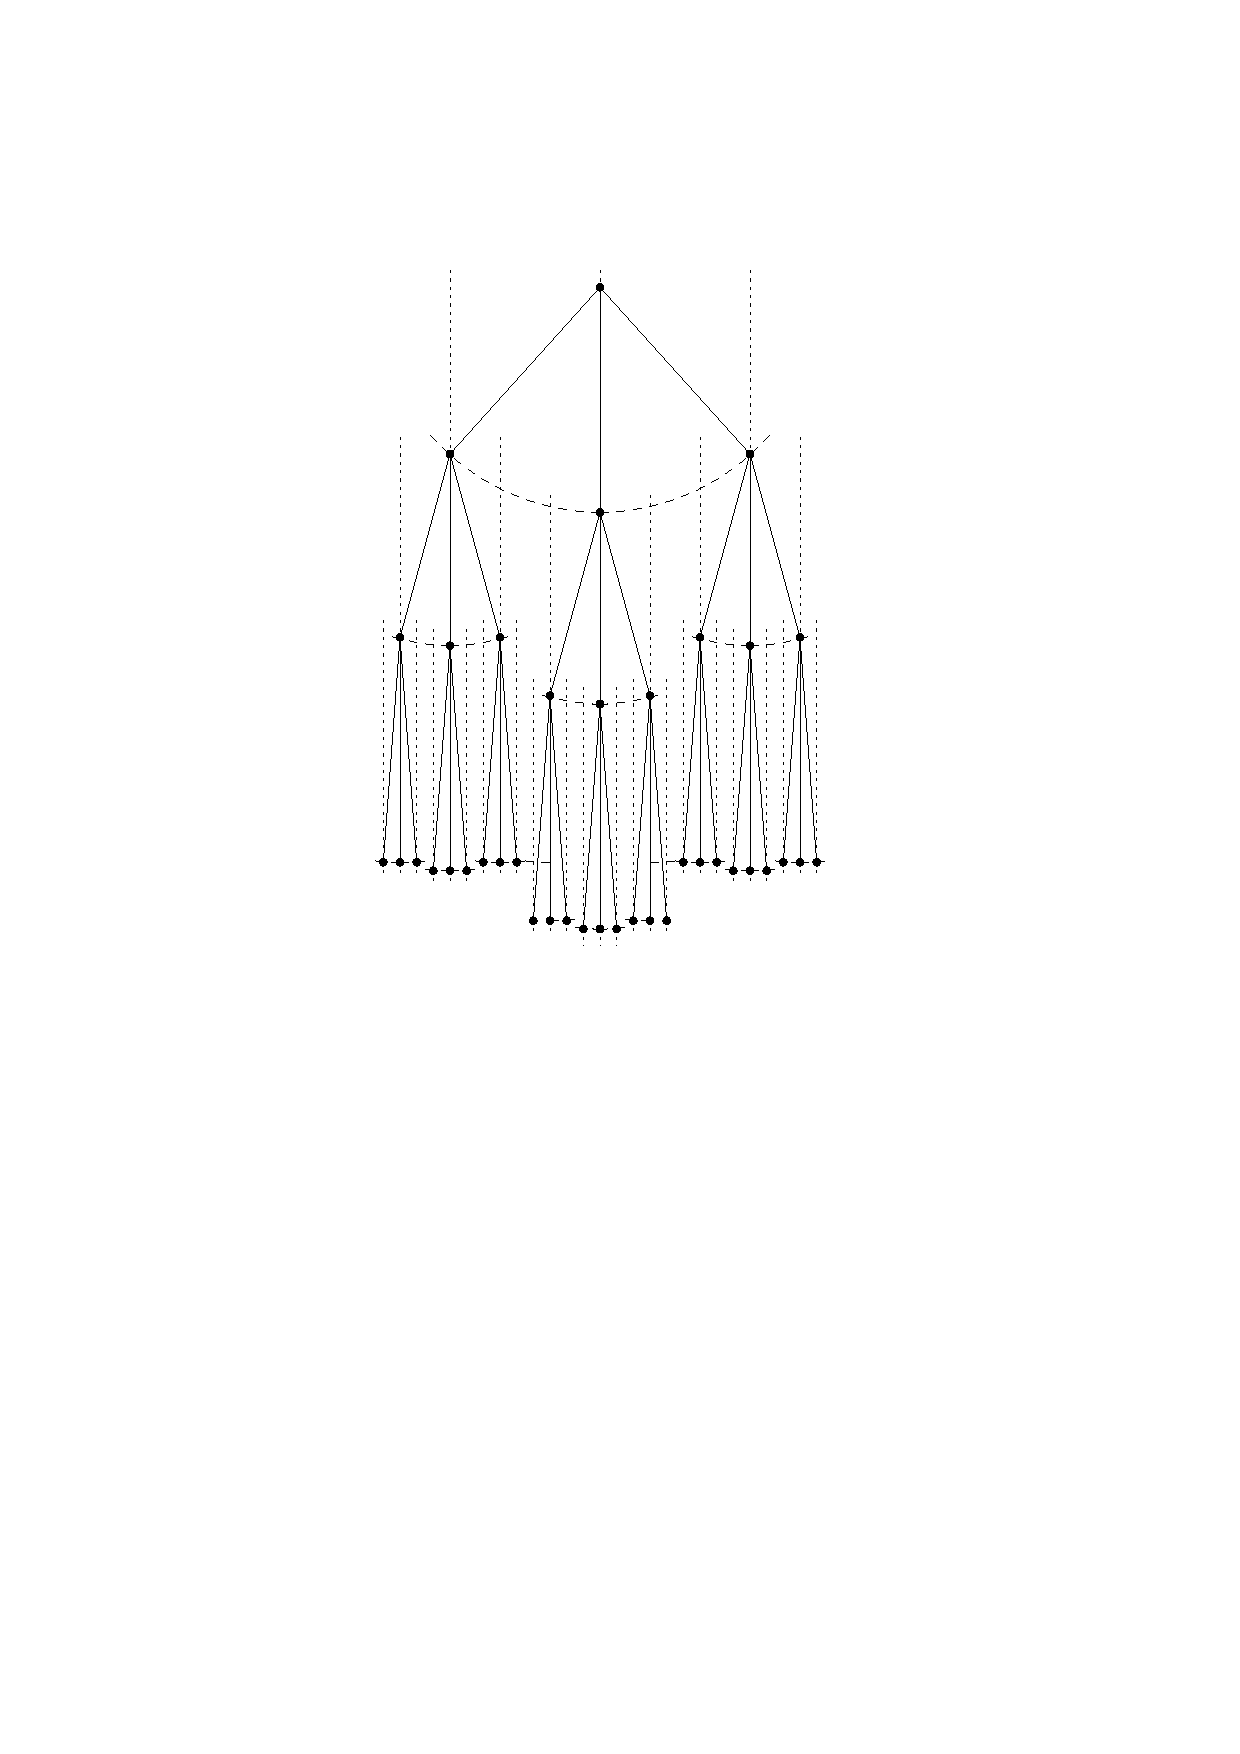
\includegraphics[page=1,width=0.6\linewidth]{graphics/k-ary_tree_example_drawings.pdf}
	\end{subfigure}
	\caption{Ternary tree with height 3}\label{im:3-ary_tree}
\end{figure}
\begin{figure}[H]
	\centering
	\begin{subfigure}{\textwidth}
		\centering
		\includegraphics[page=2,width=0.6\linewidth]{graphics/k-ary_tree_example_drawings.pdf}
	\end{subfigure}
	\caption{5-ary tree with height 2}\label{im:4-ary_tree}
\end{figure}
\begin{figure}[H]
	\centering
	\begin{subfigure}{0.5\textwidth}
		\centering
		\includegraphics[page=3,width=0.6\linewidth]{graphics/k-ary_tree_example_drawings.pdf}
	\end{subfigure}
	\caption{A rooted tree with at most 5 children per inner node}\label{im:general-tree}
\end{figure}

\subsection{Implementation}

The drawing algorithm for complete $k$-ary trees as described in this section got implemented as a script in \texttt{Python}. The \texttt{networkx} library was used to represent the graph structure. For creating a drawing, the \texttt{matplotlib} library came in handy since it allows explicite coordinate placements of vertices and a fixed aspect ratio of the resulting drawing.\\
The script consists of a \texttt{main} function and the drawing implementation of algorithm \ref{al:complete_k-ary_tree}. It is possible to set the $k$ and the height when calling the script by command-line arguments. The \texttt{main }function evaluates those command-line arguments and calls the recursive coordinate calculations starting from the root vertex with its coordinate $(0,0)$. All coordinates are rounded to integers in order to produce a straight-line drawing on a grid by default. Afterwards, the map between vertices and their coordinates are forwarded to an instance of the \texttt{matplotlib} plot. The output of the script consists of a straight-line drawing, the length of the shortest and longest edge and the ratio of the drawing.
\bigskip\\
For a full documentation of the implementation, the reader is invited to checkout the \texttt{git} repository found on $\text{GitHub}^{\copyright}$\cite{repository}.

\begin{figure}[H]
	\centering
	\begin{subfigure}{\textwidth}
		\centering
		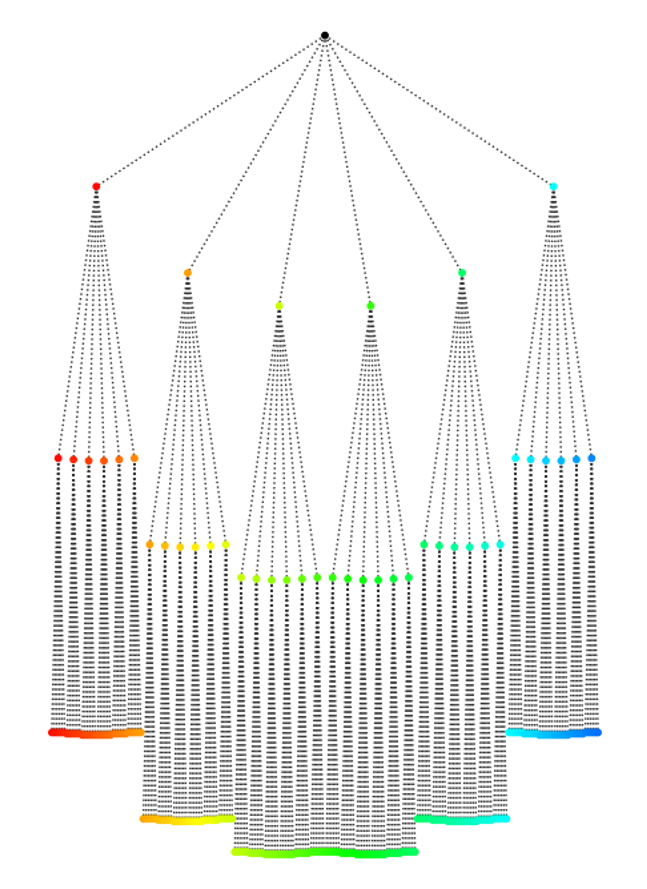
\includegraphics[width=0.7\linewidth]{graphics/Implementation_6ary_height_3ver2.png}
	\end{subfigure}
		\caption{Output drawing of a $6$-ary tree of height 3. $l_{\min}$ values 215.75, $l_{\max}$ values 216.09. The ratio values 1.0015777}
\end{figure}
\begin{figure}[H]
	\begin{subfigure}{\textwidth}
		\centering
		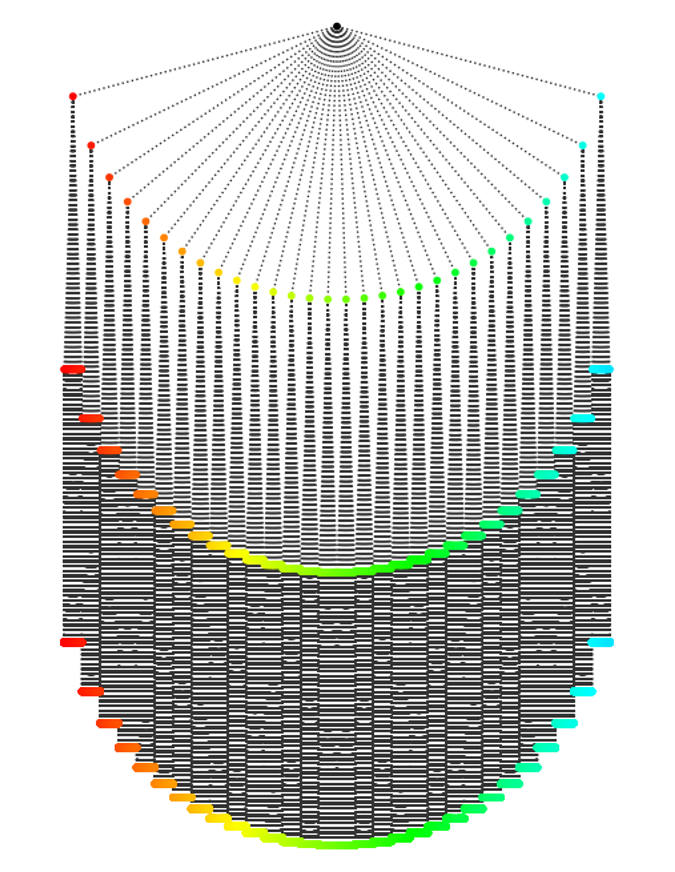
\includegraphics[width=0.7\linewidth]{graphics/Implementation_30ary_height_3ver2.png}

	\end{subfigure}
		\caption{Output drawing of a 30-ary tree of height 3. $l_{\min}$ values 26999.64, $l_{\max}$ values 27000.45. The ratio values 1.00002984}
\end{figure}
